\chapter{Analyse-Klassen-Diagramm}

In diesem Kapitel wird zuerst auf die Klassen, welche für die Implementierung nötig sind, eingegangen bevor die Abhängigkeiten zwischen diesen Klassen nochmal übersichtlich mittel eines Analyse-Klassen-Diagramms dargestellt werden.

\section{Klassen}
\begin{multicols}{2}
\begin{itemize}
    \item Kunde
    \item Adresse
    \item Vertrag
    \item Mitarbeiter
    \item Rolle
    \item Buchung
    \item Fahrzeug
    \item Fahrzeugklasse
    \item Bild
    \item Reifensatz
    \item Reifen
    \item Kennzeichen
    \item Ausrüstung
    \item Rechnung
    \item Mahnung
    \item Standort
    \item Filiale
    \item Rabattaktion
    \item Backup
    \item Hundetransportbox
\end{itemize}
\end{multicols}

\newpage

\section{Diagramm}

\begin{figure}[!ht]
    \centering
    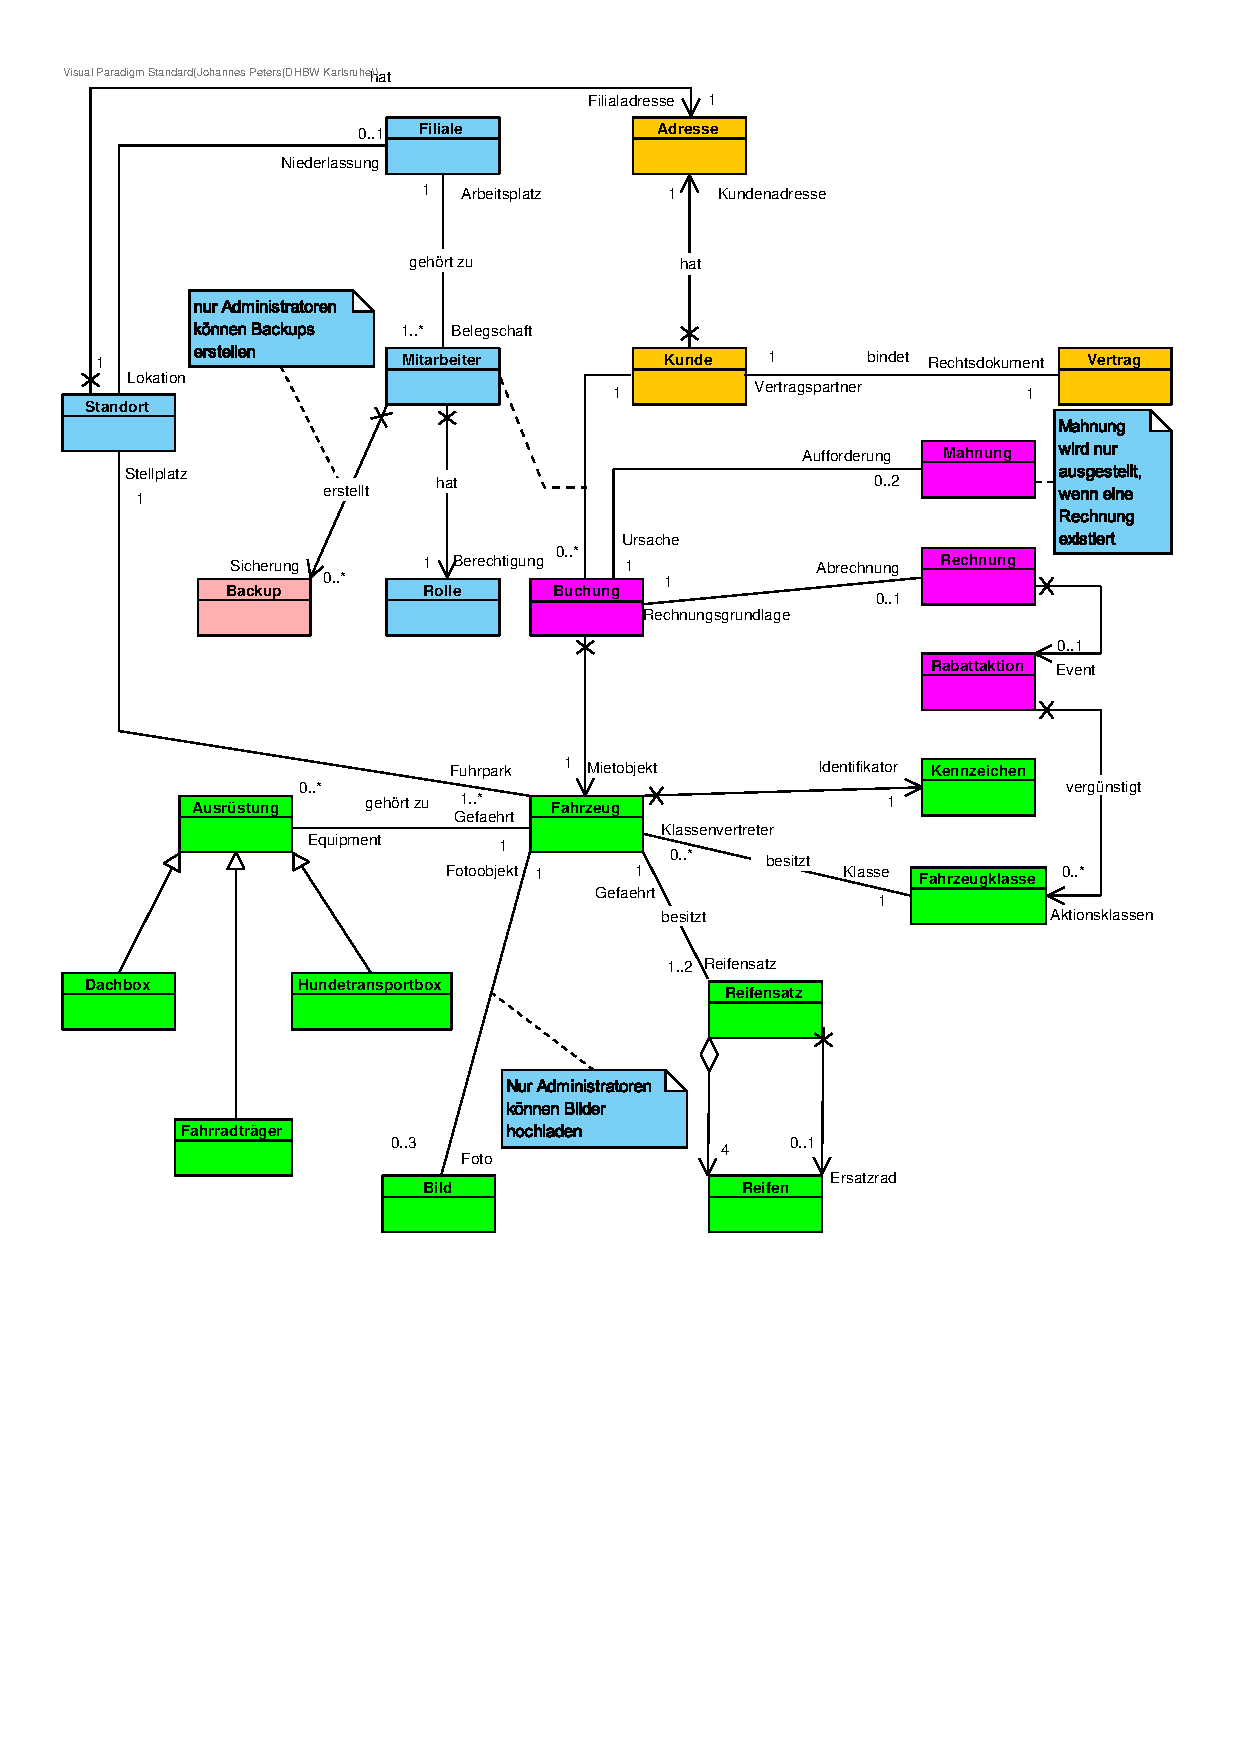
\includegraphics[width=\textwidth, trim = 0cm 9cm 0cm 0cm]{Bilder/Diagramme/Analyseklassendiagramm_v2.pdf}
    \caption{Analyseklassendiagramm}
    \label{img:akd}
\end{figure}

\newpage

\textbf{Kunde}: Sobald sich ein neuer Kunde in einer der Filialen registieren lässt, wird ein neuer Kunde angelegt. Die Kunden-Klasse führt alle nötigen Informationen zur Identifikation und Ausstellung von Rechnungen als Attribute zusammen. Von diesen Informationen sind Finanzdaten ausgenommen, da diese laut Anforderung durch ein anderes System verwaltet werden. Zu den Identifikationsinformationen gehört eine Anschrift, welche durch eine Referenz auf die Adresse-Klasse eingebracht wird. 

Dabei kann jeder Kunde nur eine Adresse haben. Umgekehrt könnte zwar auch die gleiche Adresse auf mehrere Kunden verweisen (z.B. wenn mehrere Kunden im selben Haus wohnen wie es bei einer Familie der Fall sein könnte), doch ist diese Referenz für das Programm unwichtig und somit wird die Assoziation nur unidirektional dargestellt. 

Für eine rechtliche Grundlage muss jeder Kunde einen Vertrag unterzeichnen, der digital eingescannt und abgespeichert werden soll. Die bidirektionale Verbindung weist jedem Kunden genau einen Kundenvertrag zu und natürlich wurde jeder Kundenvertrag von nur einem Kunden unterzeichnet. 

Ein Kunde kann mehrere Buchungen durchführen, die er aber zum aktuellen Projektstand nicht selbst tätigen soll. Der Kunde äußert einen Terminwunsch an einen Mitarbeiter und der Mitarbeiter legt für den Kunden eine Buchung an, die auf den Kunden verweist. Ein Kunde darf mehrere Buchungen anlegen lassen, aber eine Buchung verweist nur auf einen Kunden. Aus diesem Grund fungiert die Mitarbeiter-Klasse als Koordinator.  

\textbf{Adresse}: Die Adresse wird in Straße, Hausnummer, Wohnungszusatz, Ort und Postleitzahl aufgeteilt. Mit der Adress-Klasse werden die Adressen der Kunden und Filialen dargestellt. Da die Adresse-Klasse jeweils nur als Bestandteil anderer Klassen fungiert sind alle Assoziationen unidirektional auf die Adress-Klasse verweisend. 

\textbf{Vertrag}: Die Vertrags-Klasse bildet die Verträge ab, welche die Kunden bindet. Der Vertrag soll unterschieben eingescannt und als PDF-Datei im System abgelegt werden. Die einzigen zusätzlichen Angaben sind der Pfad und ein Vertragsdatum. Ein extra Dateiname wird nicht abgespeichert, da dieser dem Dateipfad entnommen werden kann.

\textbf{Mitarbeiter}: Die Klasse 'Mitarbeiter' stellt die Mitarbeiter des Unternehmens dar. Die Darstellung eines Mitarbeiters im System dient der Zugriffsbeschränkung der Anwendung mittels Rollen und der Identifikation von im System eingetragene Veränderungen. Jedem Mitarbeiter wird unidirektional eine Rolle zugewiesen. Da die Anwendung nicht auf Basis einer Datenbank arbeitet und auf Abfragen wie die Gruppierung der Mitarbeiter nach vergebenen Rollen irrelevant ist, wurde nur eine unidirektionale und keine bidirektionale Assoziation angenommen.

Jeder Mitarbeiter hat einen festen Arbeitsplatz, welcher durch eine Referenz auf die Klasse 'Filiale' gekennzeichnet ist. Umgekehrt sind in einer Filiale mehrere Mitarbeiter beschäftigt. 

Bereits bei der Klasse 'Kunde' angesprochen fungiert der Mitarbeiter als Koordinator zwischen Kunde und Buchung. 

Weiterhin können Mitarbeiter, unter der Einschränkung, dass der Mitarbeiter die 'Admin'-Rolle hat, Backups erstellen. Der Ausdruck 'können' impliziert, dass nicht jeder Mitarbeiter ein Backup anlegt und dass auch auch der selbe Mitarbeiter mehrere Backups erstellen kann. 

\textbf{Rolle}: Mit den Rollen sollen die Rechte innerhalb der Anwendung verteilt werden können. Dazu stellt die Klasse 'Rolle' neben dem Rollennamen auch ein Array aus Objekten, welches angibt, ob ein Nutzer mit dieser Rolle Zugriff auf die entsprechende Funktion bzw. auf eine GUI-Komponente haben soll. Die Klasse 'Rolle' referenziert keine anderen Klassen, sondern wird nur von der Klasse 'Mitarbeiter' referenziert.

\textbf{Buchung}: Die Klasse 'Buchung' stellt einen vereinbarten Termin für die Mietung eines Autos dar. Dazu wird der Mitarbeiter, welcher die Buchung angelegt hat zusammen mit dem Kunden und dem Datum sowie der Uhrzeit des Termins gespeichert. Außerdem steht die Klasse 'Buchung' in Assoziation mit der Fahrzeug-Klasse, um festlegen zu können, welches Fahrzeug gemietet werden soll. Pro Buchung soll ein Kunde nur ein einziges Fahrzeug buchen können.

Da bei einer Buchung eines Fahrzeugs der Preis durch Rabattaktionen beeinflusst werden kann, steht die Buchungs-Klasse über die Rechnung indirekt in Assoziation mit der Klasse 'Rabattaktion'. Um den Preis zufälligerweise durch mehrere Rabattaktionen nicht mehrfach zu drücken, soll pro Buchung wenn überhaupt nur eine einzige Rabattaktion einbezogen werden.

Nach Abschluss einer Fahrt bzw. nach Ablauf eines Buchungszeitraums wird automatisch eine Rechnung erstellt. Die dadurch entstehende Assoziation zwischen Buchung und Rechnung ist bidirektional. Eine Buchung weist entweder keine Rechnung vor, solange der Termin noch offen ist oder genau eine Rechnung, wenn der Termin abgeschlossen wurde.

Sofern die Rechnung im vorgegebenene Zeitrahmen beglichen wird, ist damit der Buchungsvorgang abgeschlossen, doch sollte eine Zahlung überfällig sein, erzeugt das System auf Basis der Buchung eine oder zwei Mahnungen. Jede Mahnung verweist dabei eindeutig auf die zugehörige Buchung. Eine dritte Mahnung wird nicht ausgestellt, denn anstelle dieser soll das schweizer Bankkonto eingefroren werden und andere rechtliche Schritte werden eingeleitet. 


\textbf{Fahrzeug}: Die Klasse Fahrzeuge ist für das Abbilden der Fahrzeuge zuständig und das Kernobjekt der Anwendung. Jedem Fahrzeug wird genau eine Fahrzeugklasse zugeordnet und in diesem Fall ist die Assoziation bidirektional, da umgekehrt z.B. auch eine Suche nach Fahrzeugen einer bestimmten Fahrzeugklasse möglich sein soll.

Jedes Fahrzeug im Fuhrpark des Unternehmens benötigt eine rechtlich eindeutige Identifikation mittels Nummernschild, weshalb jedes Fahrzeug auf genau ein Kennzeichen verweist. Eine umgekehrte Verknüpfung ist nicht nötig für ein einfaches Buchungssystem. 

Um die Fahrtüchtigkeit der Fahrzeuge zu allen Jahreszeiten gewährleisten zu können, müssen die Fahrzeuge mit den passenden Saisonreifen ausgerüstet sein. Um dies im Überblick zu behalten, verweist ein Fahrzeug auf einen Reifensatz. Jedes Fahrzeug hat einen Sommer- und Winterreifensatz. Um die Zuordnung zu genau dem zugehörigen Fahrzeug sicherzustellen, ist die Verbindung bidirektional. 

Für ein optisch ansprechendes GUI gibt es die Möglichkeit beim Anlegen eines neuen Fahrzeuges auch ein oder mehrere Bilder hochzuladen. Dieses Angebot ist optional und sollte kein Bild hochgeladen werden, dann wird ein 'Placeholder'-Bild eingefügt. Das Hochladen von Bildern ist nach Aufgabenanalyse und -anforderung ebenfalls als eine Administratorfunktion deklariert. Um nicht übermäßig viele Bilder hochzuladen, ist ein Limit auf drei Bilder gesetzt. 

Beim Ausleihen der Fahrzeuge für besondere Anlässe kann es auch sein, dass zusätzliche Ausrüstung erwünscht ist. Die Verbindung zur Ausrüstung ist als bidirektional gewählt, nicht nur vom Fahrzeug aus ersichtlich sein soll welche Ausrüstung vorhanden ist, sondern auch um zu verhindern, dass die selbe Ausrüstung im System ausversehen auf mehreren Fahrzeugen angebracht werden soll. 

Die letzte Assoziation für ein Fahrzeug verweist auf den Standort. Um ein Fahrzeug zu buchen, muss bekannt sein, wo dieses Fahrzeug parkt. Von der andern Seite aus betrachtet gibt es am Standort nur eine gewisse Anzahl an Parkplätzen, sodass bekannt sein muss, welche Fahrzeuge sich zu dem bestimmten Zeitpunkt vor Ort befinden. 

\textbf{Fahrzeugklasse}: Die Fahrzeugklassen sind für das Unterteilen der Fahrzeuge in verschiedene Kategorien zuständig. Diese Kategorien werden mit der Klasse 'Fahrzeugklasse' dargestellt. Eine Kategorie zeichnet sich dabei durch einen Namen, einen Preis und den benötigten Führerschein aus. Solch einer Kategorie sind beliebig viele Fahrzeuge zugeordnet. Dabei ist es denkbar, dass eine Fahrzeugklasse existiert, das Carsharing-Unternehmen aber keinen Klassenvertreter im Fuhrpark besitzt. 

\textbf{Bild}: Die Klasse Bild stellt allgemein alle Bilder in der Anwendung dar dar. Jedes Bild ist einem anderen Element (zum Beispiel Fahrzeug, Standort, ...) zugeordnet. Als weitere Attribute besitzt diese Klasse den Titel des Bildes sowie den Pfad, an welchem das Bild liegt.

\textbf{Reifensatz}: Ein Reifensatz dient der Unterscheidung zwischen Sommer- und Winterreifen und verweist auf ein bestimmtes, zugehöriges Fahrzeug, sodass jedes Fahrzeug zwei Reifensätze haben sollte. Da es z.B. auch Ganzjahresreifen gibt, kann ein Fahrzeug entweder ein oder zwei Reifensätze vorweisen.  
Jeder Reifensatz besteht aus vier Reifen und potenziell einem weiteren Reifen (Ersatzreifen).

\textbf{Reifen}: Die Klasse Reifen stellt die Reifen der Fahrzeuge dar. Ein Reifen wird hierbei durch den Hersteller, das Modell, den Zeitpunkt der Herstellung, die Profiltiefe, Saison und die Fahrtrichtung beschrieben.

\textbf{Kennzeichen}: Das Kennzeichen dient der Identifikation eines Fahrzeugs. Um das Kennzeichen eines Fahrzeugs in der Anwendung darzustellen wird die Klasse 'Kennzeichen' implementiert, welche die Zulassungsstelle, die Art des Kennzeichens und eine Zeichenkette für das eigentliche Kennzeichen als Attribute enthält.

\textbf{Rechnung}: Eine Rechnung fällt immer nach dem Abschluss einer Fahrt an. Die Klasse 'Rechnung' bildet solch eine Rechnung ab und beinhaltet Methoden um basierend auf der Buchung eine Rechnung in Form eines PDF-Dokuments zu erstellen und an den Kunden per E-Mail zu versenden. Solch eine Rechnung referenziert dabei immer auf die zugrundeliegende Buchung.

\textbf{Mahnung}: Wenn der Kunde die Rechnung nicht im vorgegebenen Zeitraum begleicht, wird eine Mahnung versendet. Die Klasse 'Mahnung' bildet solch eine Mahnung ab und beinhaltet Methoden, um basierend auf der Buchung eine Mahnung zu erstellen und um diese anschließend an den Kunden zu versenden. Ähnlich der Erstellung einer Rechnung wird ein PDF-Dokument erzeugt, welches im Fall einer Mahnung jedoch manuell ausgedruckt und mittels Post versendet wird. Da eine Mahnung stets auf einer Buchung basiert, wird die zugrundeliegende Buchung referenziert.

\textbf{Standort}: Das Unternehmen ist an verschiedensten Standorten tätig. Grundlegend ist ein Standort eine Betriebsfläche des Carsharing-Unternehmens und ist in allen Fällen eine Lokation, an der Fahrzeuge ausgeliehen werden können. Die Anzahl der Fahrzeuge ist hierbei nicht beschränkt.

Damit der Standort für die Kunden erreichbar ist, wird eine Adresse vorausgesetzt, auf die eine Klasseninstanz des Standortes wie auch bei Kunde unidirektional verweist. 

Es ist bei größeren oder wichtigeren Standorten möglich, dass sich dort auch eine Filiale des Unternehmens befindet, an die sich Kunden wenden können. Ein Standort \textbf{kann} eine Filiale referenzieren, doch umgekehrt \textbf{muss} eine Filiale allein wegen der Adressreferenz auf einen Standort verweisen.

Des Weiteren wird der Standort durch eine Beschreibung und einen Namen beschrieben. 

\textbf{Filiale}: Die Klasse 'Filiale' stellt eine Filiale des Unternehmens dar. Dafür wird die Filiale mit dem Standort in Assoziation gesetzt.

In jeder Filiale sind Mitarbeiter des Unternehmens angestellt. Das heißt, dass die Belegschaft einer Filiale mindestens ein Mitarbeiter ist, wobei theoretisch nach oben keine Schranke gesetzt ist. Als wichtige Information hat diese Klasse das Attribut 'Öffnungszeiten'. 

\textbf{Rabattaktion}: Mit der Klasse 'Rabattaktion' werden die Rabattaktionen dargestellt. Dazu besitzt diese Klasse den prozentualen Preisnachlass und den Namen der Rabattaktion als Attribute. 

Es ist möglich, dass z.B. der Rabatt nicht global auf alle Fahrzeuge gewährleistet werden soll, sondern auf einzelen oder mehrere Fahrzeugklassen. Die dabei entstehende Assoziation ist unidirektional, da eine Rabattaktion auf Fahrzeugklassen verweist, doch die Fahrzeugklasse nichts von einer Verbindung zu eine Rabattaktion kennen muss, da der Preisnachlass erst zur Rechnung erstellt wird. 

\textbf{Backup}: Die Klasse Backup ist für die Darstellung der Backups zuständig. Dafür wird zum einen das Datum und die Uhrzeit der Erstellung des Backups und zum anderen der Pfad, unter welchem das Backup abgelegt wurde, als Attribut bereitgestellt. Es gab die Überlegung, ob auch noch der Mitarbeiter verknüpft werden soll, der das Backup anlegt, doch muss diese Aufgabe nicht vom System übernommen werden, da die erstellte Backupdatei im Dateisystem diese Information des Erstellers automatisch speichert. 

\textbf{Ausrüstung}: Die Klasse 'Ausrüstung' umfasst die Ausrüstung eines Fahrzeugs. Dabei handelt es sich nicht um die Ausstattung des Fahrzeugs (Klimaanlage, Panoramaschiebedach, etc.), sondern um Zusätze wie Fahrradträger, Dachbox und Hundetransportbox. Die Klasse 'Ausrüstung' fungiert dabei als Oberklasse der Ausrüstungsgegenstände und besitzt als Attribute die Kompatibilität mit den verschiedenen Fahrzeugen und das Fahrzeug, welches den Gegenstand momentan ausgerüstet hat. Da die Ausrüstung immer einem Fahrzeug zugeordnet ist, wird stets ein Fahrzeug referenziert.

\textbf{Hundetransportbox}: Die Hundetransportbox ist eine der Unterklassen der Ausrüstung, welche die Klasse 'Ausrüstung' um folgende Attribute erweitert: Das Maximalgewicht des Hundes, Höhe, Breite und Länge sowie das Volumen.

\textbf{Fahrradträger}: Ein Fahrradträger ist ebenfalls ein Teil der Ausrüstung und somit eine Unterklasse der Klasse 'Ausrüstung'. Die Klasse Fahrradträger hat zusätzlich Attribute für die Anzahl der Fahrräder, welche mit dem Fahrradträger transportiert werden können, und das maximale Gewicht mit dem der Fahrradträger beladen werden darf.

\textbf{Dachbox}: Die letzte Unterklasse der Ausrüstung ist die Dachbox, welche zusätzlich Attribute für das Volumen und die Größenmaße der Dachbox besitzt.
